\chapter{Specifikacija rada}


\section{Specifikacija sustava}

Glavna ideja sustava je kreirati platformu za mobilno ogla\v{s}avanje. Sustav \v{c}ine mobilna aplikacija i administrativno su\v{c}elje koje bi trgova\v{c}ki lanci koristili za promociju proizvoda u svojim poslovnicama. Ideja je da trgova\v{c}ki lanaci preko internetskog su\v{c}elja kreiraju popuste za svoje proizvode u odabranim poslovinicama, a zatim kupci pomo\'{c}u mobilne aplikacije ostvaruju kreirane popuste. Korisni\v{c}ko iskustvo je zami\v{s}ljeno tako da korisnik prilikom ulaza u poslovnicu, pomo\'{c}u pametnog telefona sa instaliranom aplikacijom te NFC i BLE modulom, skenira NFC naljepnicu koja aplikaciji daje informaciju u koju je poslovnicu korisnik u\v{s}ao. Mobilna aplikacija zatim dohva\'{c}a konfiguraciju te poslovnice poslovnice sa poslu\v{z}itelja, te je ta akcija je prikazana na slici ~\ref{fig:skeniranjeNaljepnice}.

\begin{figure}[!htbp]
	\begin{center}
 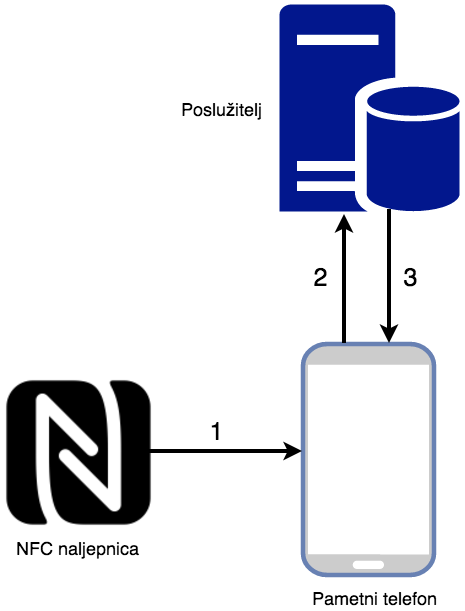
\includegraphics[height=12cm,keepaspectratio=true]{nfc_sken}
 \caption{Prikaz procesa skeniranja NFC naljepnice (1), zahtjeva za konfiguracijom poslovnice (2) i dobivanje konfiguracje poslovnice (3).}
 \label{fig:skeniranjeNaljepnice}
	\end{center}
\end{figure}

Kada aplikacija dobije konfiguraciju po\v{c}inje sa skeniranjem okoline, s ciljem nala\v{z}enja BLE ure\dj aja. Proizvodi na akciji imaju u svojoj neposrednoj blizini BLE ogla\v{s}iva\v{c} te korisniku koji prolazi pokraj police od proizvoda, ukoliko ima upaljenu aplikaciju, prona\dj eni popust postaje vidljiv u aplikaciji. Tada, ukoliko se odlu\v{c}i na iskori\v{s}tavanje popusta, kreira zahtjev za kodom popusta. Zahtjev je vezan za korisnikov ure\dj aj (zbog za\v{s}tite od zloupotrebe - svaki ure\dj aj mo\v{z}e jedan popust ostvariti maksimalno jedan put) te korisnik dobiva kod za popust kojeg je, s ciljem ostvarivanja popusta, du\v{z}an prikazati na blagajni. Opisani postupci su prikazani na slici  ~\ref{fig:otkrivanjeBLEa}.

\begin{figure}[!htbp]
	\begin{center}
 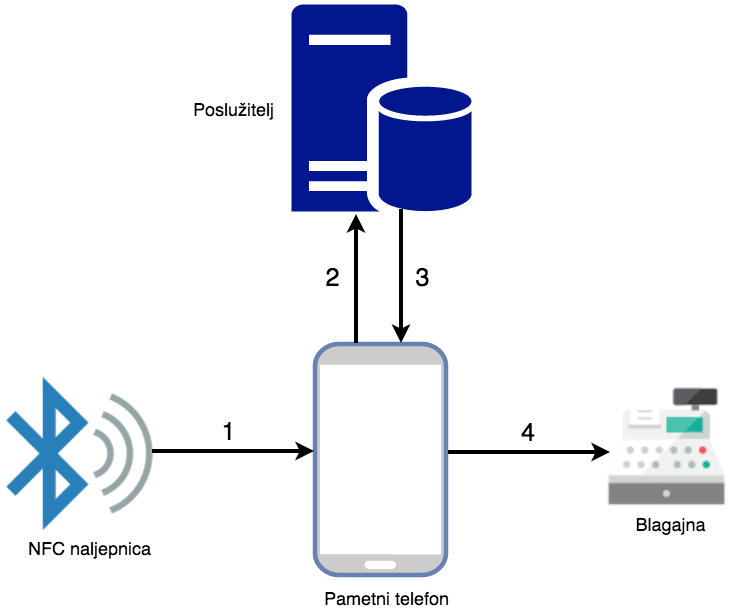
\includegraphics[height=12cm,keepaspectratio=true]{ble_sken}
 \caption{Prikaz procesa otkrivanja BLE ogla\v{s}iva\v{c}a (1), zahtjev za kodom skeniranog popusta (2), dobivanje koda za popust (3) i prikazivanje koda na blagajni za kona\v{c}no ostvarivanje popusta (4).}
 \label{fig:otkrivanjeBLEa}
	\end{center}
\end{figure}

Za implementaciju opisanog sustava potrebne su slijede\'{c}e aktivnosti:
\begin{enumerate}
	\item Kreiranje web aplikacije sa su\v{c}eljem za poslovne subjekte
	\item Kreiranje API su\v{c}elja za komunikaciju mobilne aplikacije i poslu\v{z}itelja
	\item Konfiguriranje NFC naljepnica i BLE ogla\v{s}iva\v{c}a
	\item Kreiranje mobilne aplikacije
	
\end{enumerate}

Resursi potrebni za ostvarivanje aktivnosti uklju\v{c}uju:
\begin{enumerate}
	\item NFC naljepnice
	\item BLE ogla\v{s}iva\v{c}i
	\item Pametni telefon s integriranim NFC i BLE modulom
	\item Poslu\v{z}itelj za pohranjivanje internetske aplikacije i baze podataka
\end{enumerate}


\section{Rezultati}

Rezultat ovog rada je teoretska obrada dva sli\v{c}na be\v{z}i\v{c}na protokola za prijenos podataka te sustav koji objedinjuje i NFC i BLE protokol te uz pomo\'{c}u njihovih specifi\v{c}nosti korisnicima pru\v{z}a novo i druga\v{c}ije iskustvo u obavljanju kupovine. Prakti\v{c}ni dio rada uklju\v{c}uje u potpunosti funkcionalnu internetsku i mobilnu aplikaciju. Internetska aplikacija se sastoji od dva dijela:

\begin{itemize}
	\item Su\v{c}elje za trgova\v{c}ke lance
	\begin{itemize}
		\item Implementirano dodavanje i ure\dj ivanje poslovnica
		\item Implementirano dodavanje popusta za odre\dj eni proizvod i povezivanje popusta sa odgovaraju\v{c}im ogla\v{s}iva\v{c}em
		\item Implementirano upravljanje popustima i pregledavanje iskori\v{s}tenih popusta
	\end{itemize}
	\item API su\v{c}elje
	
	\begin{itemize}
		\item Omogu\'{c}ava komunikaciju poslu\v{z}itelja i mobilne aplikacije
	\end{itemize}
\end{itemize}

Funkcionalnosti mobilne aplikacij uklju\v{c}uju:
\begin{enumerate}
	\item Skeniranje NFC naljepnica
	\item Tra\v{z}enje BLE ogla\v{s}iva\v{c}a u okolini
	\item Komunikacija sa poslu\v{z}iteljem
\end{enumerate}

U nastavku rada su opisane specifi\v{c}nosti NFC i BLE protokola, specifi\v{c}nosti tehnologija i alata pomo\'{c}u kojih je sustav kreiran, detaljan opis implementacije sustava te na poslijetku usporedba i evaluacija opisanih protokola.





